% IACR Transactions CLASS DOCUMENTATION
% Written by Gaetan Leurent gaetan.leurent@inria.fr (2016-2018)
%
% To the extent possible under law, the author(s) have dedicated all
% copyright and related and neighboring rights to this software to the
% public domain worldwide. This software is distributed without any
% warranty.
%
% You should have received a copy of the CC0 Public Domain Dedication
% along with this software. If not, see
% <http://creativecommons.org/publicdomain/zero/1.0/>.

\documentclass[preprint]{iacrtrans} 
\usepackage[utf8]{inputenc}

\setcounter{tocdepth}{4}

%% VERSION 
\newcommand{\version}{v.1.0}


%% TITLE
\title{
	
\includegraphics[width=\columnwidth]{logo_zkEVM.png} \\ \vspace{0.3cm}
  Technical Document\\ \vspace{0.3cm}	
	Recursion, aggregation and composition of proofs \\
  \version
}

\institute{}


\usepackage{caption}
\usepackage{subcaption}

% This package controls how hyperlinks are displayed
% https://es.overleaf.com/learn/latex/Hyperlinks
\usepackage{hyperref}
\hypersetup{colorlinks=true,linkcolor={red!80!black},urlcolor={blue!80!black}}

%Multiple columns
\usepackage{multicol}

% Used for super caligraphic font \mathscr{}
\usepackage{mathrsfs} 

%This ensures spaces when using ensuremath and no $$ are used to introduce math
\usepackage{xspace}

%%%%%% BEGIN OF CODE HIGHLIGHTING ENVIRONMENTS %%%%%%

%   sudo apt install texlive-latex-extra 
%   sudo apt install python-pip
%   pip install pygments
%   pip install pygments-lexer-babylon  #contains JSX
%   pip install pygments-lexer-solidity 
%   pip install pygments pygments-lexer-babylon pygments-lexer-solidity

%%%%%%% IF STATEMENTS %%%%%%%%%%%
\newif\ifPOLYGON
\POLYGONtrue

\newif\ifNOPOLYGON
\NOPOLYGONtrue


% *** COLOR COMMANDS ***
\definecolor{dblackcolor}{rgb}{0.0,0.0,0.0}
\definecolor{dbluecolor}{rgb}{0.01,0.02,0.5}
\definecolor{dgreencolor}{rgb}{0.2,0.4,0.0}
\definecolor{dgraycolor}{rgb}{0.30,0.3,0.30}
\newcommand{\dblue}{\color{dbluecolor}\bf}
\newcommand{\dred}{\color{dredcolor}\bf}
\newcommand{\dblack}{\color{dblackcolor}\bf}
\definecolor{light-gray}{gray}{0.96} %the shade of grey that stack exchange uses

%Linter for circom
\usepackage{listings}
\lstdefinelanguage{circom}[]{C}{
	morekeywords = {component, include, input, function, output, parallel, pragma, public, private, signal, template, var}, 
	sensitive=true}
\lstset{
	backgroundcolor = \color{light-gray},
	showtabs = False,
	tabsize = 2,
	showspaces = False,
	showstringspaces = False,
	commentstyle = {\ttfamily\color{dgreencolor}},
	keywordstyle = {\ttfamily\color{dbluecolor}\bfseries},
	stringstyle = {\ttfamily\color{dgraycolor}\bfseries},
	language = circom,
	basicstyle = {\fontsize{7pt}{7pt}\ttfamily},
	aboveskip = 1em,
	belowskip = 1em,
	numbers = left,%none,
	numbersep=5pt,    %space line numbers from code
	xleftmargin=2em,
	frame=single,	% adds a frame around the code
	framexleftmargin=1.7em,
	numberstyle=\tiny,%\color{gray}
	emph = {proc,retp,endp,local}, 
	emphstyle = {\color{blue}\textbf},
	literate = 	
		{<==}{{{\color{dbluecolor}<==}}}2 
		{==>}{{{\color{dbluecolor}==>{}}}}2
		{===}{{{\color{dbluecolor}==={}}}}2
		{<--}{{{\color{dbluecolor}<---{}}}}2
		{-->}{{{\color{dbluecolor}--->{}}}}2
		{*}{{{\color{dbluecolor}*{}}}}2
}

%%%%%%% END OF CODE HIGHLIGHTING ENVIRONMENTS %%%%%%%


\usepackage{tikz}
\usepackage{graphicx} % Required for including images
\usepackage[font=small,labelfont=bf]{caption}  % Required for specifying captions to tables and figures

% Copyright 2017 Sergei Tikhomirov, MIT License
% https://github.com/s-tikhomirov/solidity-latex-highlighting/

\usepackage{listings, xcolor}

\definecolor{verylightgray}{rgb}{.97,.97,.97}

\lstdefinelanguage{Solidity}{
	keywords=[1]{anonymous, assembly, assert, balance, break, call, callcode, case, catch, class, constant, continue, constructor, contract, debugger, default, delegatecall, delete, do, else, emit, event, experimental, export, external, false, finally, for, function, gas, if, implements, import, in, indexed, instanceof, interface, internal, is, length, library, log0, log1, log2, log3, log4, memory, modifier, new, payable, pragma, private, protected, public, pure, push, require, return, returns, revert, selfdestruct, send, solidity, storage, struct, suicide, super, switch, then, this, throw, transfer, true, try, typeof, using, value, view, while, with, addmod, ecrecover, keccak256, mulmod, ripemd160, sha256, sha3}, % generic keywords including crypto operations
	keywordstyle=[1]\color{blue}\bfseries,
	keywords=[2]{address, bool, byte, bytes, bytes1, bytes2, bytes3, bytes4, bytes5, bytes6, bytes7, bytes8, bytes9, bytes10, bytes11, bytes12, bytes13, bytes14, bytes15, bytes16, bytes17, bytes18, bytes19, bytes20, bytes21, bytes22, bytes23, bytes24, bytes25, bytes26, bytes27, bytes28, bytes29, bytes30, bytes31, bytes32, enum, int, int8, int16, int24, int32, int40, int48, int56, int64, int72, int80, int88, int96, int104, int112, int120, int128, int136, int144, int152, int160, int168, int176, int184, int192, int200, int208, int216, int224, int232, int240, int248, int256, mapping, string, uint, uint8, uint16, uint24, uint32, uint40, uint48, uint56, uint64, uint72, uint80, uint88, uint96, uint104, uint112, uint120, uint128, uint136, uint144, uint152, uint160, uint168, uint176, uint184, uint192, uint200, uint208, uint216, uint224, uint232, uint240, uint248, uint256, var, void, ether, finney, szabo, wei, days, hours, minutes, seconds, weeks, years},	% types; money and time units
	keywordstyle=[2]\color{teal}\bfseries,
	keywords=[3]{block, blockhash, coinbase, difficulty, gaslimit, number, timestamp, msg, data, gas, sender, sig, value, now, tx, gasprice, origin},	% environment variables
	keywordstyle=[3]\color{violet}\bfseries,
	identifierstyle=\color{black},
	sensitive=true,
	comment=[l]{//},
	morecomment=[s]{/*}{*/},
	commentstyle=\color{gray}\ttfamily,
	stringstyle=\color{red}\ttfamily,
	morestring=[b]',
	morestring=[b]"
}

\lstset{
	language=Solidity,
	backgroundcolor=\color{verylightgray},
	extendedchars=true,
	basicstyle=\footnotesize\ttfamily,
	showstringspaces=false,
	showspaces=false,
	numbers=left,
	numberstyle=\footnotesize,
	numbersep=9pt,
	tabsize=2,
	breaklines=true,
	showtabs=false,
	captionpos=b
} % Solidity Syntax highlighting package

%%%%%%%%%%%%%%%%%%% BEGIN OF MACROS %%%%%%%%%%%%%%%%%%%

% Cryptocode: https://github.com/arnomi/cryptocode
\usepackage[
lambda,
operators,
landau, %este es el de bigO
probability,
%sets,
logic, %para or,and...	
asymptotics,
keys
]{cryptocode}

% My own procedure blocks to show protocols
\createprocedureblock{mypb}{center, boxed}{}{}{linenumbering}
\createprocedureblock{mypbnonum}{center, boxed}{}{}{}

% Numbering style
\renewcommand{\pclnstyle}[1]{\text{#1}}
\renewcommand{\pclnseparator}{.}

% Hyphen inside mathmode
\mathchardef\mhyphen="2D

% Mathbb
\newcommand{\FF}{\ensuremath{\mathbb{F}}\xspace}
\newcommand{\KK}{\ensuremath{\mathbb{K}}\xspace}
\newcommand{\NN}{\ensuremath{\mathbb{N}}\xspace}
\newcommand{\ZZ}{\ensuremath{\mathbb{Z}}\xspace}

% Mathcal
\newcommand{\A}{\ensuremath{\mathcal{A}}\xspace}
\newcommand{\C}{\ensuremath{\mathcal{C}}\xspace}
\newcommand{\E}{\ensuremath{\mathcal{E}}\xspace}
\newcommand{\F}{\ensuremath{\mathcal{F}}\xspace}
\renewcommand{\H}{\ensuremath{\mathcal{H}}\xspace}
\newcommand{\I}{\ensuremath{\mathcal{I}}\xspace}
\renewcommand{\O}{\ensuremath{\mathcal{O}}\xspace}
\renewcommand{\P}{\ensuremath{\mathcal{P}}\xspace}
\newcommand{\R}{\ensuremath{\mathcal{R}}\xspace}
\renewcommand{\S}{\ensuremath{\mathcal{S}}\xspace}
\newcommand{\T}{\ensuremath{\mathcal{T}}\xspace}
\newcommand{\V}{\ensuremath{\mathcal{V}}\xspace}

% Mathscr
% \newcommand{\PPP}{\ensuremath{\mathscr{P}}\xspace}


% Mathfrak
\newcommand{\afr}{\ensuremath{\mathfrak{a}}\xspace}
\newcommand{\bfr}{\ensuremath{\mathfrak{b}}\xspace}

% Caligraphic Combiantions
\DeclareMathAlphabet{\mathpgoth}{OT1}{pgoth}{m}{n}
\newcommand{\plonk}{\ensuremath{\mathcal{P}\mathfrak{lon}\mathcal{K}}\xspace}
\newcommand{\plookup}{\ensuremath{\mathpgoth{plookup}}\xspace}

% Abbreviations
% \newcommand{\Pp}{\ensuremath{\mathcal{P}_{\textsf{poly}}\xspace}}
\newcommand{\MTR}{\ensuremath{\text{MTR}}\xspace}
\newcommand{\MTP}{\ensuremath{\text{MTP}}\xspace}
\newcommand{\LCC}{\ensuremath{\text{LCC}}\xspace}
\newcommand{\FRI}{\ensuremath{\textsf{F}}\xspace}
\newcommand{\z}{\ensuremath{\overline{z}}\xspace}
\newcommand{\fsel}{\ensuremath{f^{\text{sel}}}\xspace}
\newcommand{\tsel}{\ensuremath{t^{\text{sel}}}\xspace}
\newcommand{\Evals}{\ensuremath{\textsf{Evals}}\xspace}
\newcommand{\pparams}{\ensuremath{\text{pp}}\xspace}
\newcommand{\vparams}{\ensuremath{\text{vp}}\xspace}
\newcommand{\pre}{\ensuremath{\text{pre}}\xspace}
\newcommand{\tr}{\ensuremath{\text{tr}}\xspace}
\newcommand{\otr}{\ensuremath{\overline{\text{P}}}\xspace}
\newcommand{\im}{\ensuremath{\text{im}}\xspace}
\newcommand{\seed}{\ensuremath{\textsf{seed}}\xspace}
\newcommand{\transcript}{\ensuremath{\textsf{transcript}}\xspace}
\newcommand{\AIR}{\ensuremath{\textsf{A}}\xspace}
\newcommand{\eAIR}{\ensuremath{\textsf{eA}}\xspace}
\newcommand{\accept}{\ensuremath{\textsf{accept}}\xspace}
\newcommand{\reject}{\ensuremath{\textsf{reject}}\xspace}
\newcommand{\eFRI}{\ensuremath{\epsilon_{\textsf{FRI}}}\xspace}
\newcommand{\eSTARK}{\ensuremath{\epsilon_{\textsf{STARK}}}\xspace}
\newcommand{\eeSTARK}{\ensuremath{\epsilon_{\textsf{eSTARK}}}\xspace}
\newcommand{\eC}{\ensuremath{\epsilon_{\textsf{C}}}\xspace}
\newcommand{\ePlo}{\ensuremath{\epsilon_{\textsf{Plo}}}\xspace}
\newcommand{\eMulEq}{\ensuremath{\epsilon_{\textsf{MulEq}}}\xspace}
\newcommand{\eCon}{\ensuremath{\epsilon_{\textsf{Con}}}\xspace}
\newcommand{\eArgs}{\ensuremath{\epsilon_{\textsf{Args}}}\xspace}
\newcommand{\RS}{\ensuremath{\textsf{RS}[\FF,H,\rho]}\xspace}
\newcommand{\RSK}{\ensuremath{\textsf{RS}[\KK,H,\rho]}\xspace}
\newcommand{\LH}{\ensuremath{\textsf{LH}}\xspace}
\newcommand{\ID}{\ensuremath{\textsf{ID}}\xspace}

% Caligraphic Combiantions
 \DeclareMathAlphabet{\mathpgoth}{OT1}{pgoth}{m}{n}

% Abbreviations
\newcommand{\stoc}{\texttt{S2C}\xspace}
\newcommand{\ctos}{\texttt{C2S}\xspace}


% Make a nice emptyset
\let\oldemptyset\emptyset
\let\emptyset\varnothing

% Make a nice phi and epsilon
\let\oldphi\phi
\let\phi\varphi
\let\oldepsilon\epsilon
\let\epsilon\varepsilon

% Make a nice q.e.d. symbol
\renewcommand\qedsymbol{\ensuremath{\blacksquare}\xspace}

\theoremstyle{definition}
\newtheorem{protocol}{Protocol}
\newtheorem{bremark}{Remark}

\usepackage{paralist} % for compactitem environment

%%%%%%%%%%%%%%%%%%% END OF MACROS %%%%%%%%%%%%%%%%%%%

% \begin{pcvstack}[boxed, center]
% % \pcsetargs{codesize=\scriptsize{}}

% \procedure{}{
%   \textbf{Prover } \P(g_1(x))  \< \< \textbf{verifier } \V(g_1(x)) \\[][\hline]
%   \< \sendmessageright{top={$f_1(s)$, $f_2(s)$}} \< \\[-2mm]
%   \< \sendmessageleft{top={randomness}} \< \\[-2mm]
%   \< \sendmessageright{top={$f_3(s)$}} \< \\[-2mm]
%   \< \< \text{Samples a random } z \in \FF \text{ and computes } z\vec{g}. \\[-2mm]
%   \< \sendmessageleft{top={$z$}} \< \\[-2mm]
%   \text{Computes evaluations:} \< \< \\
%   \t g_1(z), f_1(z), f_2(z), f_3(z) \< \< \\[-2mm]
%   \< \sendmessageright{top={$g_1(z)$, $f_1(z)$, $f_2(z)$, $f_3(z)$}} \< \\[-2mm]
%   \< \sendmessageleft{top={$v$}} \< \\[-2mm]
%   \< \sendmessageright{top={$\pi$}} \< \\[-2mm]
%   \< \< \text{Verifies the opening proof } \pi \text{ and checks that:} \\
%   \< \< \t g_1(z)(f_1(z) + f_2(z)) - f_3(z) = 0
% }
% \end{pcvstack}

\newcommand{\definedir}[2]{\newcommand{#1}{#2}}
\definedir{\recursiondir}{..}

\newif\ifBACKGROUND

\begin{document}
\begin{titlepage}
\centering
\maketitle
\today
\end{titlepage}

% use optional argument because the \LaTeX command breaks the PDF keywords
% \keywords[\publname, ToSC, TCHES, LaTeX]{TBD \and TBD}

{\hypersetup{linkcolor=.}\tableofcontents}

\newpage
\section{Introduction}

Blockchain interoperability refers to the ability of a blockchain to interchange data with other blockchains. Since the blockchain ecosystem has expanded rapidly in recent years, a large number of networks with different specific properties have emerged and interoperability has become a crucial consideration in blockchain design. Without interoperability, a network risks being isolated from the larger ecosystem and this fact has supposed an incentive to projects to engage the research and development of interoperability solutions. Multiple approaches have been implemented in order to solve the problem, each one of them with particular trade offs and underlying technologies. This document describes the solution implemented by the Polygon team to bring native interoperable properties to the Polygon zkEVM L2 network.

The bridge is an infrastructure component that allows migration of assets and communication between L1 and L2. From the point of view of the user, they should be able to transfer an asset from one network to another without changing its value or its functionality, as well as being able to send data payloads between networks (cross-chain messaging).

In L2 rollups as Polygon zkEVM, the management of the L2 State transitions and the data availability of transactions is secured by L1 contracts, hence with a correct design of the L2 architecture we can also synchronize both ends of the a bridge relying only in contract's logic, without the need of off-chain trusted reliers to sync the bridge's ends across networks. It's important to note that this type of bridge must be included into the design of the L2 layer.

As can be seen in figure 1, the bridging interface is a bridge contract instance present in both networks whereby users will be able bridge assets (1), that is, lock an asset in "origin" network, and eventually, claim an asset's representative token that will be minted by the bridge contract in "destination" network. The reverse operation will be possible as well (2) , that is, to burn the asset's representative token and unlock the original asset in "origin" network. Another possible usage is as cross-chain communication channel (3), that is, to send a data payload from  L1 to L2 or vice versa.

\begin{center}
	\includegraphics[scale=0.27]{\bridgedir/figures/l2-bridge.png}
	
	\captionof{figure}{Polygon zkEVM bridge schema.}
\end{center}


%Nevertheless, its design is scalable and could be implemented to interconnect $n$ L2 between them, and at the same time, with the L1 on which they run.




%Although in its most general expression the type of bridge proposed could interconnect multiple networks, for simplicity, during this article we will focus on the analysis of the structure of a bridge that interconnects L1  with only one L2.

 

%In the specific case of the Polygon zkEVM Bridge, when the asset to be bridged is ether, no token representer will be minted, instead, will be transferred as network native asset, that is, the token used to pay transaction gas.

%\begin{center}
%\includegraphics[scale=0.27]{l2-bridge.png}

%\captionof{figure}{Polygon multi L2 bridge schema.}
%\end{center}

\section{Exit Merkle trees}

The bridge system is composed of a Merkle tree known as the Global Exit Merkle Tree (GEMT). In this tree, every leaf node represents the Merkle root of a specific network Exit Merkle Tree (EMT). The GEMT has only two leaves, one corresponding to the root of the L1 EMT , and the other corresponding to the root of the L2 EMT. Figure 2 shows the structure of the GEMT.
%Hence, GEMT will have as many leaves as networks interconnect the bridge. In our specific case, since we are analysing the particular case of only one L2 connected, our

\begin{center}
	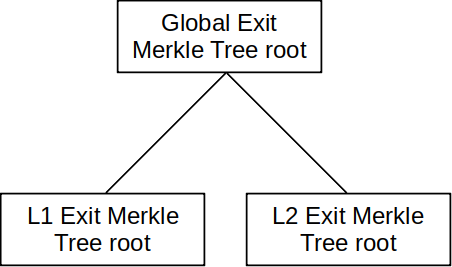
\includegraphics[scale=0.27]{\bridgedir/figures/gemt.png}
	
	\captionof{figure}{GEMT structure.}
	
\end{center}

While GEMT is a fixed 2 leaves regular Merkle tree, EMT are append only sparse Merkle trees (SMT) with a fixed depth (32 in Polygon zkEVM). SMT are massive Merkle trees that can be handled in an efficient way on-chain (detailed in appendix A). 

Every leaf of specific network EMT will represent an intention of bridge an asset (or asset's representative token) or send a message out of that network. Specifically the leaf will be a keccak256 hash of the abi encoded packed structure of the following parameters:

\begin{itemize}
	\item \textbf{uint8 leafType:} [0] asset, [1] message.
	\item \textbf{int32 originNetwork:} Origin Network ID, where the original asset belongs.
	\item \textbf{address originAddress:} If leaf type = 0, Origin network token address, "0x0000...0000" address is reserved for ether. If leaf type = 1 msg.sender of the message.
	\item \textbf{uint32 destinationNetwork:} Bridging destination network ID.
	\item \textbf{address destinationAddress:} Address that will receive the bridged asset in the destination netwok.
	\item \textbf{uint256 amount:} Amount of tokens/ether to brige.
	\item \textbf{bytes32 metadataHash:} Hash of the metadata. Metadata will contain information about asset transfered or the message payload.
\end{itemize}

Once a leaf has been added to EMT, a new EMT root will be computed, and subsequently, a new GEMT root. The GEMT root will be synced between networks, making it possible to prove leaf inclusion on the second network and complete the bridge operation.

\section{Contracts Architecture}

Most of the bridge architecture is implemented using smart contracts on both networks. However, to synchronize GEMT among them, a portion of the bridge logic must be integrated with the L2 State management architecture. So that, to provide a comprehensive description of the bridge, one must take into account the off-chain actors involved in L2 state management, including a Sequencer, an Aggregator, and the \textbf{PolygonZkEVM.sol} contract.

In addition to the previously mentioned components, the following components are also included in the bridge architecture:

\begin{itemize}
	\item \textbf{PolygonZkEVMBridge.sol:} bridging interface, allows users to interact with the bridge and perform actions such as bridging and claiming assets or messages. It has an instance in each network and manages its EMT.
	\item \textbf{PolygonZkEVMGlobalExitRoot.sol:} Manages the GEMT, which involves storing the tree and computing new root values every time a new EMT is updated by the PolygonZkEVM.sol contract (updates L2 EMT) or the L1 PolygonZkEVMBridge.sol contract (updates L1 EMT). Acts as GEMT historical repository.
	\item \textbf{PolygonZkEVMGlobalExitRootL2.sol:} Special contract that allows the synchronization of GEMT and L2 EMT roots across networks. Has storage slots to store GEMT roots and L2 EMT root. This contract is special because its storage slots are directly accessed by the low-level zero-knowledge proving/verification system to ensure the validity of GEMT synced from L1 to L2, and the validity of L2 EMT synced from L2 to L1.


\end{itemize}

\subsection{Bridging data flows.}

Figure 3 shows the detailed architecture of the bridge and how the components interact with each other to achieve finality in bridge operations. As can be seen, depending on whether the bridge operation is from L1 to L2 (L1 -> L2) or from L2 to L1 (L2 -> L1), there are two possible data flows. 

\begin{center}
	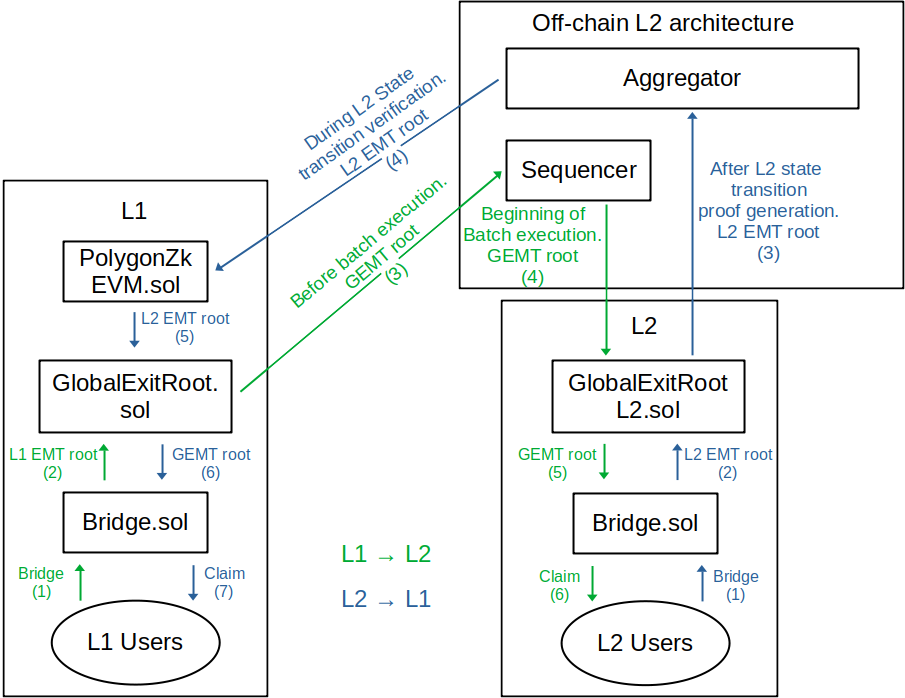
\includegraphics[scale=0.34]{\bridgedir/figures/architecture.png}
	
	\captionof{figure}{Polygon zkEVM bridge architecture.}
	
\end{center}

The steps involved in each execution flow are enumerated and explained below:

\textbf{L1 -> L2:}
\begin{itemize}
	\item \textbf{(1):} The user have to call the bridging function of the L1 \textbf{PolygonZkEVMBridge.sol} contract. Depending on the type of asset to be bridged the contract internals will act different. If the bridging request is valid, the contract will fill the L1 EMT leaf based on the characteristics of the request, add it into the tree, and compute the new L1 EMT root.
	\item \textbf{(2):} In the same L1 transaction the \textbf{PolygonZkEVMBridge.sol} contract will call the \textbf{PolygonZkEVMGlobalExitRoot.sol} contract to update the new L1 EMT root and consequently compute the new GEMT root.
	\item \textbf{(3):} Eventually, the Sequencer will fetch the new GEMT root to from \textbf{PolygonZkEVMGlobalExitRoot.sol} contract.
	\item \textbf{(4):} The new GEMT root will be entered in the special storage slots of the \textbf{PolygonZkEVMGlobalExitRootL2.sol} contract at the beginning of transaction batch execution, allowing L2 users to access it. 
	\item \textbf{(5) \& (6):} To complete the bridging process, users must call the claiming function of the L2 \textbf{PolygonZkEVMBridge.sol} contract and provide it with a Merkle inclusion proof of the leaf that was included previously. The contract will retrieve the GEMT root from the \textbf{PolygonZkEVMGlobalExitRootL2.sol} contract and verify the validity of the inclusion proof. If the inclusion proof is valid, the contract will finish the bridging process differently depending on the type of asset being bridged. If the inclusion proof is not valid, the transaction will be reverted.

\end{itemize}

\textbf{L2 -> L1:}
\begin{itemize}
	\item \textbf{(1):} The user have to call the bridging function of the L2 \textbf{PolygonZkEVMBridge.sol} contract. Depending on the type of asset to be bridged the contract internals will act different. If the bridging request is valid, the contract will fill the L2 EMT leaf based on the characteristics of the request, add it into the tree, and compute the new L2 EMT root.
	\item \textbf{(2):} In the same L2 transaction the \textbf{PolygonZkEVMBridge.sol} contract will call the \textbf{PolygonZkEVMGlobalExitRootL2.sol} contract to update the new L2 EMT.
	\item \textbf{(3):} Eventually, the Aggregator will generate the Zero-Knowledge proof of computational integrity of the execution of the sequence of batches in which the bridging transaction is included. The new L2 EMT will be obtained from the L2 state that results from the execution.
	\item \textbf{(4):} The Aggregator will submit the resulting L2 EMT, along with the Zero-Knowledge proof to the L1 \textbf{PolygonZkEVM.sol} contract.
	\item \textbf{(5):} \textbf{PolygonZkEVM.sol} contract will verify the validity of the Zero-Knowledge proof and, if it is valid, the contract will call \textbf{PolygonZkEVMGlobalExitRoot.sol} contract to update the new L2 EMT root and consequently compute the new GEMT root.
	\item \textbf{(6) \& (7):} To complete the bridging process, users must call the claiming function of the L1 \textbf{PolygonZkEVMBridge.sol} contract and provide it with a Merkle inclusion proof of the leaf that was included previously. The contract will retrieve the GEMT root from the \textbf{PolygonZkEVMGlibalExitRoot.sol} contract and verify the validity of the inclusion proof. If the inclusion proof is valid, the contract will finish the bridging process differently depending on the type of asset being bridged. If the inclusion proof is not valid, the transaction will be reverted.
\end{itemize}



\subsection{PolygonZkEVMBridge.sol}


\textbf{PolygonZkEVMBridge.sol} is the contract that acts as a bridging interface for users in a specific network, hence has an instance in each network. Has the storage slots required to hold the EMT of each network and all necessary functions to interact with it.
\subsubsection{Bridging functions}
% Manages the EMT of each network, that is, stores Branch array (B$_{x}$) needed to manage the incremental Merkle tree on-chain and has all necessary functions to interact with the tree.
\textbf{bridgeAsset} is the function used to bridge assets out  to another network:

\begin{lstlisting}[language=solidity]
	function bridgeAsset(
        address token,
        uint32 destinationNetwork,
        address destinationAddress,
        uint256 amount,
        bytes calldata permitData
    )
\end{lstlisting}

\textbf{bridgeAsset function arguments:}

\begin{itemize}
	\item \textbf{token:} ERC20 token address in origin network, if its "0x0000...0000" means that the user wants to bridge ether.
	\item \textbf{destinationNetwork:} Network ID of the destination network, must be different of the network ID in which is called the function, otherwise the transaction will revert.
	\item \textbf{destinationAddress:} Address that will receive the bridged tokens in the destination netwok.
	\item \textbf{amount:} Amount of tokens to bridge
	\item \textbf{permitData:} Signed permit data for ERC-20 tokens with EIP-2612 Permit extension, used to change an account's ERC-20 allowance, and permit the brige contract to transfer to himself the tokens to be bridged.
	
\end{itemize}

As can be seen in figure 4, since there are three different types of assets that can be bridged, there are three possible execution flows for the \textbf{bridgeAsset} function:

\begin{itemize}
	\item \textbf{(1) The asset to be bridged is ether.}
	\item \textbf{(2) The asset is a representative ERC-20 token of an ERC-20 token from another network.}
	\item \textbf{(3) The asset is an ERC-20 token original from this network.}
\end{itemize}

\begin{center}
	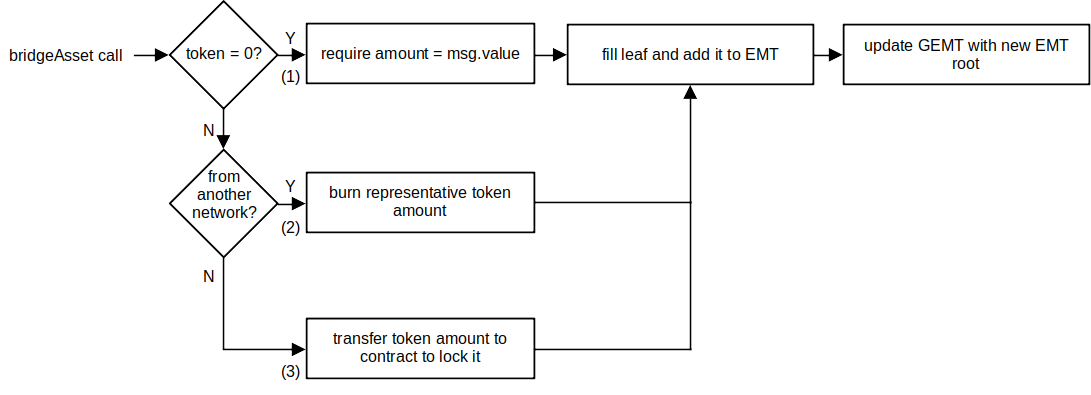
\includegraphics[scale=0.40]{\bridgedir/figures/bridge-asset.png}
	
	\captionof{figure}{Possibles execution flows of \textbf{bridgeAsset} function depending on the type of the asset.}
	
\end{center}



\textbf{(1) The asset to be bridged is ether:}

If the \textbf{token} argument equals to "0x0000...0000" means that the asset to bridge is ether, and the msg.value of the transaction shall match with the \textbf{amount} argument. The ether amount will be locked in the contract in order to proceed with the bridging process. Note that the ether in L1 and in L2 is treated in the same way, indeed, it is bridged with 1:1 exchange ratio and will be the gas payment (native) token in both networks. Since ether is original from L1 the leaf's parameter \textbf{originNetwork} will be set to L1 network ID. 

\textbf{(2) The asset is a representative ERC-20 token of an ERC-20 token from another network:}

Representative ERC-20 tokens are managed by the \textbf{PolygonZkEVMBridge.sol} contract, which is responsible for minting and burning them. Additionally, the contract has a mapping named \textbf{wrappedTokenToTokenInfo} that acts as a list of representative ERC-20 token contracts deployed on this network. For each contract representative token deployed, this mapping will have an entry following the \textbf{TokenInformation} struct, with the address of representative token contract as the key.

\begin{lstlisting} [language=Solidity]
	struct TokenInformation {
		uint32 originNetwork;
		address originTokenAddress;
	}
\end{lstlisting}
If the \textbf{token} argument value is present as a key in the \textbf{wrappedTokenToTokenInfo} mapping, it means that the token being bridged is a representative ERC-20 token of an ERC-20 token from another network. In order to proceed with the bridging process, a quantity of  token corresponding to the \textbf{amount} argument will be burned, the bridge has the rights to burn the tokens without the user's allowance. Leaf's parameters, \textbf{originAddress} and \textbf{originNetwork}, will be taken from the \textbf{wrappedTokenToTokenInfo} mapping's corresponding entry.

\textbf{(3) The asset is an ERC-20 token original from this network:}

The last possible flow occurs when the assets to be bridged are ERC20 tokens originals from this network. In this case, in order to proceed with the bridging process, a quantity of token corresponding to the \textbf{amount} argument will be locked in the contract. Note that to successfully transfer the tokens to himself, the contract must have allowance over at least the quantity of tokens that the user wants to bridge. If the token contract supports EIP-2612 permit extension the allowance can be also done in the same transaction giving the signed \textbf{permitData} argument. Leaf's parameters, \textbf{originNetwork} and \textbf{originTokenAddress}, will be set to the current network ID and ERC-20 token contract address, respectively. The \textbf{metadataHash} parameter of the leaf will also be computed as follows. This parameter will ensure that the representative ERC-20 token contract is deployed with exactly the same ERC-20 token parameters in the destination network.

\begin{lstlisting}[language=Solidity]
	 metadataHash = keccak256(
	 	abi.encode(
			IERC20MetadataUpgradeable(token).name(),
			IERC20MetadataUpgradeable(token).symbol(),
			IERC20MetadataUpgradeable(token).decimals()
		)
	);
\end{lstlisting}



The last execution step is common regardless the type of asset.
The remaining leaf's parameters, \textbf{leafType}, will be set to 0 (type asset) and \textbf{destinationNetwork} and \textbf{destinationAddress} will be set according to the arguments of the \textbf{bridgeAsset} function call. First, a \textbf{BridgeEvent} event that contains all the information of the leaf will be emitted. Then, the new leaf will be included in the EMT. Finally, the GEMT contract will be called to update the new EMT root.

\vspace{0.5cm}

\textbf{bridgeMessage} is the function used to bridge a message to another network:

\begin{lstlisting}[language=solidity]
	function bridgeMessage(
        uint32 destinationNetwork,
        address destinationAddress,
        bytes memory metadata
    )
\end{lstlisting}

\textbf{bridgeMessage function arguments:}

\begin{itemize}
	\item \textbf{destinationNetwork:} Network ID of the destination network, must be different of the network ID in which is called the function, otherwise the transaction will revert.
	\item \textbf{destinationAddress:} Address in the destination network that will receive the bridged message.
	\item \textbf{metadata:} Message payload.
\end{itemize}

\textbf{bridgeMessage} function will directly emit a \textbf{BridgeEvent} event, will add a new leaf to the EMT and will call GEMT to update the new EMT root as \textbf{bridgeAsset} function does. The main difference is that the leaf it creates is of type message (leafType = 1), hence, \textbf{orginAddress} and \textbf{metadataHash} leaf's values will be the msg.sender and the hash of the message payload respectively. The user can bridge ether along with the message by simply adding the amount as the msg.value in the \textbf{bridgeMessage} function call transaction, this amount will be sent as value when \textbf{destinationAddress} will be called to receive the message in the destination network.

\subsubsection{Claiming functions}

Since L2 accounts, by default, do not have ether to pay transaction fees, when claiming bridged assets or messages from L1, L2 claiming transactions that call bridge claiming functions are funded by the protocol and will not require the payment of gas fees.

\textbf{claimAsset} is the function used to claim assets bridged from other networks:

\begin{lstlisting}[language=solidity]
	function claimAsset(
        bytes32[] memory smtProof,
        uint32 index,
        bytes32 mainnetExitRoot,
        bytes32 rollupExitRoot,
        uint32 originNetwork,
        address originTokenAddress,
        uint32 destinationNetwork,
        address destinationAddress,
        uint256 amount,
        bytes memory metadata
    )
\end{lstlisting}

\textbf{claimAsset function arguments:}

\begin{itemize}
	\item \textbf{smtProof:} Merkle proof, that is, the sibling nodes array needed to verify the leaf.
	\item \textbf{index:} Index of the leaf.
	\item \textbf{mainnetExitRoot:} L1 EMT root when the leaf has been included.
	\item \textbf{rollupExitRoot:} L2 EMT root when the leaf has been included.
	\item \textbf{originNetwork:} Origin Network ID, where the original asset belongs.
	\item \textbf{originTokenAddress:} ERC20 token address in origin network, if its 0x0000..0000 means that ether is being claimed.
	\item \textbf{destinationNetwork:} Network ID of the destination network, that is, the network where the call is being made.
	\item \textbf{destinationAddress:} Address that will receive the bridged tokens.
	\item \textbf{amount:} Amount of tokens that are claimed.
	\item \textbf{metadata:} If the asset being claimed is not original from the network where the call is being made the ABI encoded metadata of the original ERC-20 token (name, symbol, decimals) will be used as metadata. If is either Ether or a token original from the network where the call is being made, the value would be 0.
\end{itemize}


The \textbf{claimAsset} function will verify the validity of the leaf that corresponds to the arguments provided by the user.
	 		
To prevent replay attacks, measures should be taken to ensure that a given leaf can only be successfully verified once. \textbf{PolygonZkEVMBridge.sol} contract has a \textbf{claimedBitMap} mapping to store a nullifier bit for each leaf index that has already been successfully verified. As can be seen in figure 5, in order to optimize storage slots usage, each entry in the mapping will hold 256 nullifier bits for 256 already verified leaves.
	
	\begin{center}
		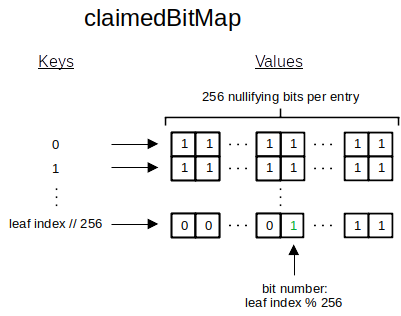
\includegraphics[scale=0.65]{\bridgedir/figures/nullifier.png}	
		\captionof{figure}{\textbf{claimedBitMap} nullifier mapping structure.}
	\end{center}
	
In order for a Merkle proof of a specific leaf to be considered valid, the following conditions must be met:
	\begin{itemize}
		\item The leaf's nullifying bit must be unset in \textbf{claimedBitMap} mapping.
		\item The leaf's \textbf{destinationNetwork} parameter must match the network ID in which the \textbf{claimAsset} function is being called.
		\item The GEMT root resulting of hashing \textbf{mainnetExitRoot} and \textbf{rollupExitRoot} arguments must already exist in the \textbf{PolygonZkEVMGlobalExitRoot.sol} contract.
		\item The Merkle proof must be valid, which means it should produce the expected GEMT root.
	\end{itemize}
	
	  
If the leaf is successfully verified, the leaf index will be nullified by setting its corresponding bit in \textbf{claimedBitMap} mapping, and then, as can be seen in figure 6, since there are three different types of assets that can be claimed, there are three possible execution flows for the \textbf{claimAsset} function:
	
\begin{itemize}
	\item \textbf{(1) The asset to be claimed is ether.}
	\item \textbf{(2) The asset is an ERC-20 token original from this network.}
	\item \textbf{(3) The asset is a representative ERC-20 token of an ERC-20 token from another network.}
\end{itemize}
	
\begin{center}
	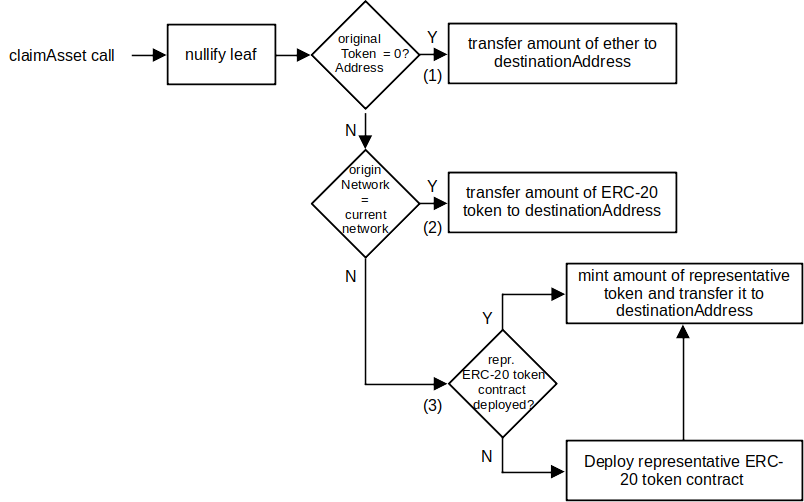
\includegraphics[scale=0.40]{\bridgedir/figures/claim-asset.png}
		
	\captionof{figure}{Possibles execution flows of \textbf{bridgeAsset} function depending on the type of the asset.}
	
\end{center}
	
\textbf{(1) The asset to be claimed is ether:}

if the \textbf{originTokenAddress} argument equals to "0x0000...0000" means that the asset that is being claimed is ether, hence a transaction with the value of \textbf{amount} argument quantity of ether will be sent to \textbf{destinationAddress} argument address.
Since ether cannot be minted on demand, \textbf{PolygonZkEVMBridge.sol} deployed on L2 has a balance of preminted 100000000000 ether as ether bridging liquidity. It is assumed that all ether in L2 is bridged form L1 so, L1's \textbf{PolygonZkEVMBridge.sol} does not need to have ether balance beforehand, every ether wei in L2 will have a backing ether wei blocked in L1 contract. Note that the preminted liquidity of L2 \textbf{PolygonZkEVMBridge.sol} does not have any inflationary effect on ether.
	
\textbf{(2) The asset is an ERC-20 token original from this network:}
	
If the \textbf{originNetwork} argument equals to the network ID where the call is being made, it means that the asset being claimed is original from that network and should already be locked in the balance of \textbf{PolygonZkEVMBridge.sol} contract. Hence, the \textbf{amount} argument quantity of ERC-20 tokens will be sent to \textbf{destinationAddress} argument address.

	
\textbf{(3) The asset is a representative ERC-20 token of an ERC-20 token from another network:}
	
The last possible flow occurs when the assets that is being claimed is an ERC20 token original from another network.

The \textbf{PolygonZkEVMBridge.sol} contract has a mapping called \textbf{tokenInfoToWrappedToken} which stores the addresses of representative ERC-20 token contracts deployed on the network. The salt used during the deployment of the contracts using the create2 function is used as a key in each entry of the mapping.
	
The salt is computed as follows from the \textbf{originNetwork} and \textbf{originTokeAddress} arguments:
	
\begin{lstlisting}[language= Solidity]
	keccak256(
		abi.encodePacked(originNetwork, originTokenAddress)
	);
\end{lstlisting}
	
The contract will check if the representative ERC-20 token contract for the asset being claimed is present in the \textbf{tokenInfoToWrappedToken} mapping. If it is, it means that the representative ERC-20 token contract has already been deployed, and the quantity specified in the \textbf{amount} argument will be minted to the address specified in the \textbf{destinationAddress} argument.
	
If it is not present, a new representative ERC-20 token contract will be deployed using the create2 function and the previously computed salt. The use of the create2 function and this specific salt will deterministically bind the address of the representative token contract to the address of the original token contract on origin network. Then, the quantity specified in the \textbf{amount} argument will be minted to the address specified in the \textbf{destinationAddress} argument, and a \textbf{NewWrappedToken} event will be emitted. 
	
A new entry in \textbf{tokenInfoToWrappedToken} and \textbf{wrappedTokenToTokenInfo} mappings will be added for the new representative ERC-20 token contract.

	
Finally, regardless of the kind of asset being claimed, a \textbf{ClaimEvent} event will be emitted.

\vspace{0.5cm}
	
\textbf{claimMessage} is the function used to claim messages bridged from other networks:
	
	
\begin{lstlisting}[language=solidity]
	function claimMessage(
        bytes32[] memory smtProof,
        uint32 index,
        bytes32 mainnetExitRoot,
        bytes32 rollupExitRoot,
        uint32 originNetwork,
        address originAddress,
        uint32 destinationNetwork,
        address destinationAddress,
        uint256 amount,
        bytes memory metadata
    )
\end{lstlisting}


\textbf {claimMessage}, as \textbf{claimAsset} function does, will try to verify the leaf given by the user, since the leaf format is the same, both functions will take the same arguments. And again, as \textbf{claimAsset} function does, if the leaf is successfully verified the leaf index will be nullified by setting its corresponding bit in \textbf{claimedBitMap} mapping.
Then, low level call will be made to \textbf{destinationAddress} argument as the follows:

\begin{lstlisting}[language=Solidity]
// Execute message
// Transfer ether
/* solhint-disable avoid-low-level-calls */
(bool success, ) = destinationAddress.call{value: amount}(
	abi.encodeCall(
		IBridgeMessageReceiver.onMessageReceived,
		(originAddress, originNetwork, metadata)
	)
);
\end{lstlisting}

As can be seen, call data is set in order to call a function \textbf{onMessageReceived} passing \textbf{originAddress}, \textbf{originNetwork}, \textbf{metadata} arguments, if the message contains  ether, call value will be set to \textbf{amount} argument. \textbf{metadata} will be the message payload. Note that messaging service can be used to transfer ether to Externally owned accounts (EOAs), however the message cannot be interpreted by them hence the message payload will be unusable.

Finally, if the message sending succeeds, a \textbf{ClaimEvent} event will be emitted.


\subsection{PolygonZkEVMGlobalExitRoot.sol}


\textbf{PolygonZkEVMGlobalExitRoot.sol} is the L1 contract that computes and store each new GEMT root. In order for any added leaves to be verifiable in the future, every GEMT root needs to be stored. A mapping named \textbf{globalExitRootMap} holds all computed GEMT roots. L1 \textbf{PolygonZkEVMBridge.sol} will fetch the GETM roots form this mapping during the leaf verification process.

As can be seen in figure 7, the \textbf{updateExitRoot} function is used to update the values of EMT roots and compute a new GEMT root. If it is called by the \textbf{PolygonZkEVM.sol} contract, the L2 EMT root will be updated. If it is called by the \textbf{PolygonZkEVMBridge.sol} contract, the L1 EMT root will be updated. This function will accept only cal
ls coming  from \textbf{PolygonZkEVM.sol} or from \textbf{L1 PolygonZkEVMBridge.sol} contract.
\begin{lstlisting} [language=Solidity]
	function updateExitRoot(bytes32 newRoot) external 
\end{lstlisting}

\begin{center}
	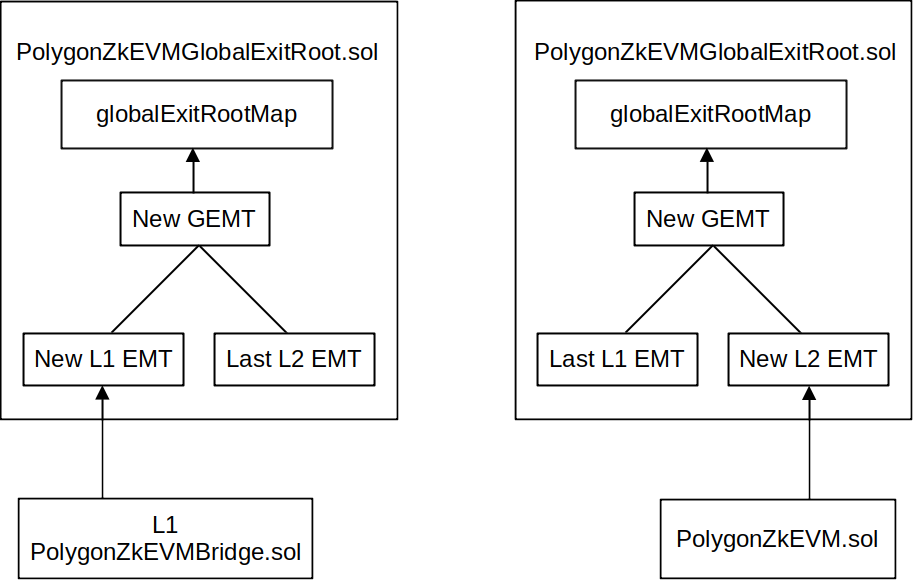
\includegraphics[scale=0.3]{\bridgedir/figures/gemt-update.png}
	
	\captionof{figure}{Two execution flows of \textbf{updateExitRoot} function.}
	
\end{center}


When each L2 state transition is consolidated by the \textbf{PolygonZkEVM.sol} contract (through ZK proof verification given by the Aggregator), a new L2 EMT will be updated in the \textbf{PolygonZkEVMGlobalExitRoot.sol} contract through a call to the \textbf{updateExitRoot} function.

With each new leaf added to L1 EMT \textbf{PolygonZkEVMBridge.sol} contract, a new L1 EMT root will need updated in the \textbf{PolygonZkEVMGlobalExitRoot.sol} contract, so on \textbf{PolygonZkEVMBridge.sol} will call \textbf{updateExitRoot} function in order to update the new L1 EMT root.

Finally an event \textbf{UpdateGlobalExitRoot} will be emitted.

\subsection{PolygonZkEVMGlobalExitRootL2.sol}

\textbf{PolygonZkEVMGlobalExitRootL2.sol} is a "special" contract deployed in L2 that allows to L2 \textbf{PolygonZkEVMBridge.sol} instance to have access to GEMT roots history. Note that L2 \textbf{PolygonZkEVMBridge.sol} instance cannot directly call L1 \textbf{PolygonZkEVMGlobalExitRoot.sol} contract to query GEMT roots since it is deployed in another network.

\textbf{PolygonZkEVMGlobalExitRootL2.sol} as \textbf{PolygonZkEVMGlobalExitRoot.sol} has the mapping \textbf{globalExitRootMap} to store the GEMT roots, but instead of compute them by itself the \textbf{globalExitRootMap} mapping is synchronized between networks regarding the mapping in L1 \textbf{PolygonZkEVMGlobalExitRoot.sol} contract.

\textbf{PolygonZkEVMGlobalExitRootL2.sol} stores last L2 EMT root value updated by L2 \textbf{PolygonZkEVMBridge.sol} instance every time that a new leaf is added to L2 EMT.

\textbf{PolygonZkEVMGlobalExitRootL2.sol} is "special" because \textbf{globalExitRootMap} and \textbf{lastRollupExitRoot} storage slots are directly accessed by the zkEVM node SW during the transactions batches execution. 

In order to allow to the L2 users to claim assets bridged, \textbf{globalExitRootMap} must be synchronized by zkEVM node at the beginning of the batch execution, then L2 \textbf{PolygonZkEVMBridge.sol} contract will have access to the valid GEMT roots to verify users claim transactions contained in the batch.

L2 EMT root is queried form \textbf{lastRollupExitRoot} variable by zkEVM node that acts as Aggregator after the execution of the batches. Then the L2 EMT root will be sent along with the L2 State transition proof to L1 \textbf{PolygonZkEVM.sol} contract, and if the proof verification succeeds, it will update the new L2 EMT root in L1 \textbf{PolygonZkEVMGlobalExitRoot.sol} contract and the new GEMT will be computed to allow to L1  \textbf{PolygonZkEVMBridge.sol} contract to have access to the valid GEMT roots to verify users claim transactions contained in the aggregated batches.


\appendix

\section{Gas efficient append only sparse Merkle tree}

A sparse Merkle tree is a Merkle tree of an intractable size that can be handled in an efficient way, making the assumption that it is almost empty, indeed, initially it is empty. It is considered empty when all leaves in it have the same zero (empty) value, thanks to this assumption it is possible to calculate the root by computing $log_{2}(n)$ hash operations where $n$ is the number of leaves on the tree. Note that in a non-sparse tree we will need to compute $2n-1$ hash operations to compute the root. During the computation of the empty tree root, in each level all nodes will take the same value, hence it is not needed to compute all subtrees in every level. Every value that takes a node in a specific level of the tree when it is empty is named Zero Hash and will represent a subtree of $x$ zero leaves. 


For example, for an empty sparce Merkle of 3 levels (8 leaves), the Zero Hash list will be as follows:
\begin{itemize}
	\item level 0 node = 0
	\item level 1 node = H(0,0) = ZH$_{1}$
	\item level 2 node = H(ZH$_{1}$,ZH$_{1}$) = ZH$_{2}$
	\item level 3 node  = H(ZH$_{2}$,ZH$_{2}$) = ZH$_{3}$ = Merkle root
	
\end{itemize}

\begin{center}
	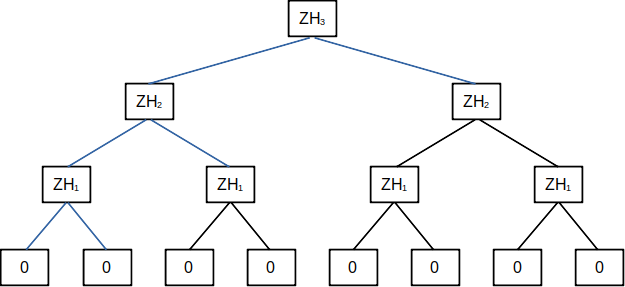
\includegraphics[scale=0.35]{\bridgedir/figures/empty-smt-example.png}
	
	\captionof{figure}{8 leaves empty sparse Merkle tree.}
\end{center}

To add new values to the tree we will use only $1  + log_{2}(n)$ hash operations, in addition to ZH evaluations if we do not have them precomputed. Indeed compute ZH on the fly is more gas efficient than reading storage slots with the precomputed values. Every new value added will fill one empty leaf of the tree. 

Continuing with the previous example, to add first value (L$_{0}$) we will compute the following hash operations:
\begin{itemize}
	\item H(L$_{0}$)   = B$_{0}$
	\item H(B$_{0}$,0) = B$_{1}$
	\item H(B$_{1}$,ZH$_{1}$) = B$_{2}$
	\item H(B$_{2}$,ZH$_{2}$) = Merkle root
\end{itemize}

\begin{center}
	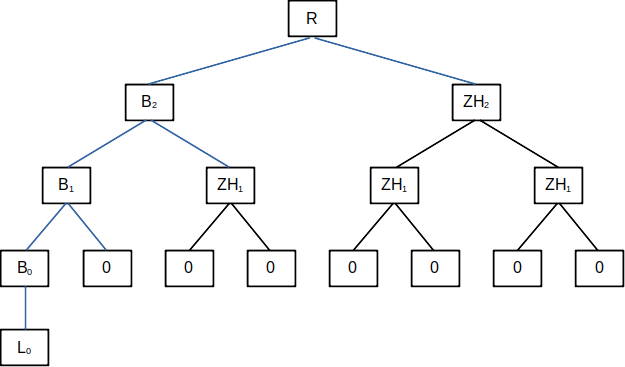
\includegraphics[scale=0.35]{\bridgedir/figures/l0-smt-example.png}
	
	\captionof{figure}{8 leaves sparse Merkle tree first leave inclusion.}
\end{center}

Note that we are computing a $n$ leaves Merkle root, using only $1 + log_{2}(n)$ hash operations, and we will have the same situation for any leaf added consecutively. B$_{x} $ (Branch) are all the values of the already computed subtrees, and it will be the storage slots needed to store the tree on-chain. So the whole storage slots needed to implement an incremental Sparce Merkle tree on-chain will be $ 1 + log_{2} (n) $.

Regarding the inclusion proof verification operations there is no difference between a regular Merkle tree and a sparse one, it can continue to be done efficiently using $1 + log_{2}(n)$ hash operations. In addition, to generate the inlcusion proof, it will be nedded to have access to all the already included leves of the tree, nevertheless it is not needed to use storage slots since we have it available in the inclusion transaction calldata or by the emission of an event during the inclusion.

To sum up, SMT are massive Merkle trees that can be handled in an efficient way, and can be stored using a few storage slots. Efficiency in terms of on-chain computation means less transactions gas cost as well as low storage usage.

\section{Bridging flows}
\subsection{L1 -> L2}

\begin{center}
	\includegraphics[scale=0.175]{\bridgedir/figures/out/l1-l2-bridge-flow/data-exchange-resolution-k.png}
	
	\captionof{figure}{L1 -> L2 bridging flow.}
	
\end{center}

\subsection{L2 -> L1}

\begin{center}
	\includegraphics[scale=0.175]{\bridgedir/figures/out/l2-l1-bridge-flow/data-exchange-resolution-k.png}
	
	\captionof{figure}{L2 -> L1 bridging flow.}
	
\end{center}


\ifNOPOLYGON
\section{Questions}
\textbf{Why EMT are SMT with 32 levels?}

\textbf{The GEMT is synced to L2 in a non deterministic way, are there any check to protect to a bad sequencer to set a invalid GEMT?}

Since the GEMT is checked during the sequencing stage of the protocol, an invalid GEMT will only be valid in the trusted L2 State stage. Transaction batches that include an invalid GEMT can never be sequenced, as the sequencing transaction will revert. This means that there can never be a virtual or consolidated state with an invalid GEMT.


\section{TODO}
\begin{itemize}
	\item use plant UML bridging flows?
	\item intro to bridges.
\end{itemize}
\fi

\newpage
\bibliographystyle{alpha}
\bibliography{bib/bibliography,cryptobib/abbrev3,cryptobib/crypto}

\newpage
\appendix

\end{document}